\chapter{有监督学习}
\label{chap:supervised}
机器学习分为:监督学习,无监督学习。
本章先介绍\emph{监督学习}(supervised learning),
它从给定的训练数据集中学习出一个函数,用于对新数据的预测。
监督学习的训练集包括输入和输出,也即是特征和目标。
训练集中的目标是由人标注的,利用这些已知数据和其输出训练得到一个最优模型(目标函数)。
监督学习是训练神经网络和决策树的常见方法。
最典型的算法是KNN和SVM,用于回归分析和统计分类。

\section{训练过程}
有监督学习最常见的就是:回归(Regression)和分类(Classification)。
一般来说,定量输出称为回归,或是对连续变量预测;
定性输出称为分类,就是对离散变量进行预测。K-近邻(KNN)是一种分类算法,
而之前提到的线性回归,就是利用已知数据集求线性函数,使其尽可能地拟合数据,
也就是让损失函数最小。

\section{回归问题}
回归分析分为:线性回归、逻辑回归(Logistic Regression)。
实际上,逻辑回归就是对线性回归的输出又进行了一次特殊函数的处理,
使其输出一个分类可能性的概率,这个特殊的函数通常是sigmoid函数:
$$ y = \frac{1}{1+e^{-x}} $$
\begin{figure}[!htbp]
\centering
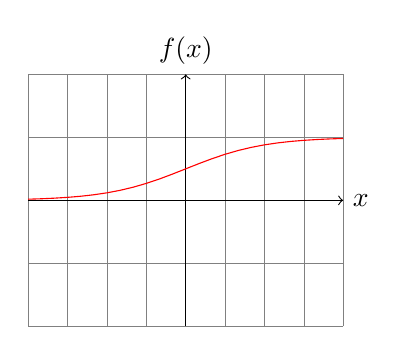
\begin{tikzpicture}[yscale=0.8, xscale=0.5]
  \draw[very thin,color=gray] (-4,-2) grid (4,2);
  \draw[->] (-4,0) -- (4,0) node[right] {$x$};
  \draw[->] (0,-2) -- (0,2) node[above] {$f(x)$};
	\draw[color=red, domain=-4:4] plot (\x,{1/(1+e^-\x)});
\end{tikzpicture}
\end{figure}

Sigmoid函数是机器学习非常重要的一个函数,
当$x>0$时,Sigmoid函数大于0.5;当$x<0$时,Sigmoid函数小于0.5。
因此,把拟合曲线的函数值带入Sigmoid函数,
比较$f(x)$与0.5的大小就可判断其分类。
总的来说,Sigmoid函数具有以下几个良好性质:
\begin{enumerate}
	\item 单调可微,具有对称性。
	\item 便于求导。
	\item 定义域为$[-\infty, +\infty]$,值域为$(0, 1)$,可将任意值映射为概率。
\end{enumerate}

\subsection{线性回归}
之前章节介绍过线性回归的数学模型,并尝试用梯度下降法,找到线性函数的参数,来拟合数据集。
所以实现线性回归的代码,得首先实现梯度的算法函数,分为:SGB、BGD和MBGD。

因为\emph{批梯度下降}是使用所有的数据样本拟合出来的假设函数,
所以计算梯度也就会涉及到所有的样本数据,这种情况就是所谓的BGD(Batch Gradient Descent)。
结合最小二乘法的定义,定义损失函数
$J(\theta)=\frac{1}{2}\sum_i^m(y_i-h_\theta(x^i))^2$
现在问题就转化为求解最优的$\theta$,使损失函数$J(\theta)$取最小值。

$$ \theta_j:=\theta_j-\alpha\frac{\delta}{\delta\theta_j}J(\theta) $$

我们先随便给$\theta$一个初始化的值(多默认为1),然后改变$\theta$值让J($\theta$)的取值变小,
不断重复改变$\theta$使$J(\theta)$变小的过程直至$J(\theta)$约等于最小值。
此算法也称为\emph{最小均方算法}(Least mean square,LMS算法)。
$$ \theta_j:=\theta_j+\frac{1}{\alpha}\sum_i^m (y_i-h_\theta(x^i))x^i_j $$
\noindent
使用伪代码表示如下,:
\begin{lstlisting}[escapeinside=``]
repeat{    
	`$ \theta_j:=\theta_j+\frac{1}{\alpha}\sum_i^m (y_i-h_\theta(x^i))x^i_j $`
  for every j=0, ... , n)
}
\end{lstlisting}

\noindent
其中$\alpha$称为步长(learning rate),控制$\theta$每次向$J(\theta)$变小的方向迭代的幅度。
由以上伪代码,也容易发现BGD(\emph{批梯度下降})每次迭代都得把所有样本计算一次,计算量很大。
把整个过程分解一下,包含:初始化、求偏导和梯度下降。
\vspace{0.3cm}

\noindent
Java代码,大致如下。
\begin{lstlisting}[language=Java, escapeinside=``]
	// `$h(x) = \theta_0 * x_0 + \theta_1* x_1 + \theta_2 * x_2$`
	public class LinearRegression {
		public LinearRegression(double[][] data,double alpha,int iteration){}

		private void     initialize_theta(){}
		public  void     train(){}
		private double[] partial_derivative(){}
		private double   partial_derivative_of_theta(int j){}
		private double   h_theta_x_i_minus_y_i_times_x_j_i(int i,int j){}
	}
\end{lstlisting}



\subsection{逻辑回归}
Sigmoid的其中一个优点就是容易求解导数,利于编码实现。
推导过程略,相应的实现代码如下:
$$ y = \frac{1}{1+e^{-x}}, y' = y*(1-y) $$

\begin{lstlisting}[language=Java]
	public static double sigMoid(double value) {
		double e_x = Math.pow(Math.E, -value);
		double result = 1 / (1 + e_x);
		return result;
	}

  public static double sigMoidDerivative(double value) {
		double A = sigMoid(value);
		double B = 1 - sigMoid(value);
		double result = A * B;
		return result;
  }
\end{lstlisting}


\section{SVM}
在机器学习章节中,我们提到过利用SVM(支持向量机)作为数据分类的一种方法,并提到了
SVM的实质其实就是正确分类数据的直线,并且分类直线与支持向量的间隔较远。在这样的基础
上,我们有必要对坐标系内点与直线的距离进行研究。假设$\mathbf{w_{i}}$为分类直线
的函数,$\delta_{i}$代表坐标与分类直线的距离,$\mathbf{\|\mathbf{w}\|}$代表向量
$\mathbf{w}$的范数\footnote{范数是对向量长度的度量,如果一个向量可以表示为
$\mathrm{W}=(w_1, w_2, w_3, \ldots ,w_n)$,那么该向量的范数则为
$\|w\|_{n}=\sqrt[n]{m_{1}^{p}+m_{2}^{n}+...+w_{n}^{n}}$},由此我们可以得到一般性的点到直线距离公式:

\begin{equation}
	\boldsymbol{\delta}_{i}=\frac{1}{\|\mathbf{w}\|}\left|g\left(x_{i}\right)\right|
\end{equation}

在二维坐标中,利用解析几何的知识,我们可以将公式简化为更容易理解的形式:
$D=(Ax+By+c) / \sqrt{A^{2}+B^{2}}$,
其中$Ax+By+c$就相当于$g(x_{i})$,$\sqrt{A^{2}+B^{2}}$相当于$\mathbf{w}$的范数。
这个公式的代码实现如下:
$$ ax + by + c = 0 $$

\begin{lstlisting}[language=Java]
	public double getDistance(double x, double y){
        double denominator = a * x + b * y + c;
        double numerator = Math.sqrt(a * a + b * b);
        double result = denominator / numerator;
        return result;
    }
\end{lstlisting}

在界定了分隔直线后,空间就被分成了$g(x_{i}) > 0$和$g(x_{i}) < 0$
两个部分,以此便可以判断数据类型的不同。与此同时,根据我们在机器学习章节
中提出的要求,最佳直线应该与所有支持向量等距且最远;因此,我们我们需要对最佳
直线与支持向量间的距离进行研究。

\begin{figure}[!ht]
    \begin{center}
    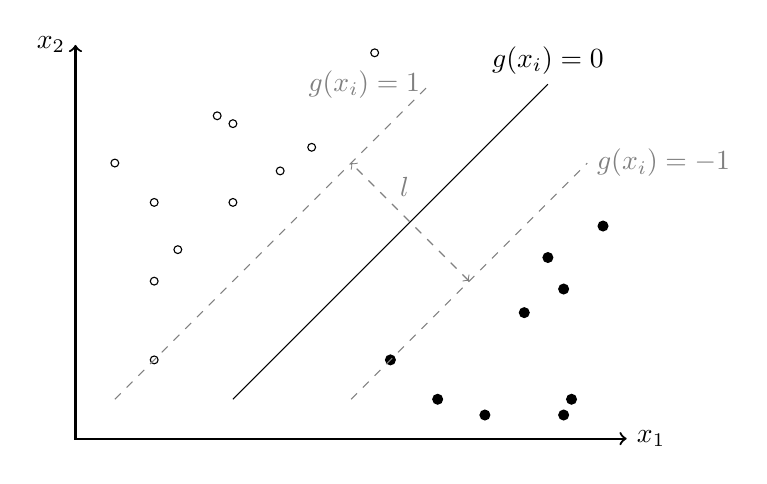
\begin{tikzpicture}
        \pgfmathsetmacro{\ticker}{0.125}
        \draw [<->,thick] (0,5) node (yaxis) [left] {$x_2$}
				|- (7,0) node (xaxis) [right] {$x_1$};
		\node[draw,circle,inner sep =1pt] (A) at (1,3) {};
		\node[draw,circle,inner sep =1pt] (B) at (0.5,3.5) {}; 
		\node[draw,circle,inner sep =1pt] (C) at (1,2) {}; 
		\node[draw,circle,inner sep =1pt] (D) at (1,1) {}; 
		\node[draw,circle,inner sep =1pt] (E) at (2,4) {};
		\node[draw,circle,inner sep =1pt] (F) at (2,3) {};
		\node[draw,circle,inner sep =1pt] (G) at (1.3,2.4) {};
		\node[draw,circle,inner sep =1pt] (H) at (3,3.7) {};
		\node[draw,circle,inner sep =1pt] (I) at (3.8,4.9) {};
		\node[draw,circle,inner sep =1pt] (J) at (2.6,3.4) {};
		\node[draw,circle,inner sep =1pt] (K) at (1.8,4.1) {};
		\fill[black] (4,1) circle (2pt);
		\fill[black] (4.6,0.5) circle (2pt);
		\fill[black] (5.2,0.3) circle (2pt);
		\fill[black] (5.7,1.6) circle (2pt);
		\fill[black] (6,2.3) circle (2pt);
		\fill[black] (6.2,1.9) circle (2pt);
		\fill[black] (6.7,2.7) circle (2pt);
		\fill[black] (6.3,0.5) circle (2pt);
		\fill[black] (6.2,0.3) circle (2pt);
		\draw[dashed, color=gray, domain=0.5:4.5]    plot (\x,{1 * \x}) node[left]{$g(x_{i}) = 1$};
		\draw[color=black, domain=2:6]    plot (\x,{1 * \x - 1.5}) node[above]{$g(x_{i}) = 0$};
		\draw[dashed, color=gray, domain=3.5:6.5]    plot (\x,{1 * \x - 3}) node[right]{$g(x_{i}) = -1$};
		\draw[dashed, color=gray, <->] (5,2)--(3.5,3.5) node[right] at (4, 3.2){$l$};
        \end{tikzpicture}
		\label{SVM_supersurface_picture}
		\caption{二维向量的线性分类器}
    \end{center}
\end{figure}

在这里,我们构建了名为“线性分类器”的模型来解决这一问题,如图\ref{SVM_supersurface_picture}。
这个问题的关键在于比较支持向量与分类直线的距离,那么我们不妨设当$g(x_{i}) > 0$
时,直线上方的支持向量经过直线$g(x_{i}) = 1$;同理,$g(x_{i}) < 0$时,直线下方
的支持向量经过直线$g(x_{i}) = -1$,这样假设方便我们进行进一步的处理。我们可以得出
$g(x_{i}) = 1$和$g(x_{i}) = -1$间的距离,即$l = 2 /\|w\|$。同时,SVM的目标是在对数据进行
正确分类的情况下,最大化分类直线和支持向量的距离;由此,我们可以得到以下关系:

$$y_{i}\left(w x_{i}-b\right)>=1$$
$$\max(2 /\|w\|)$$

可以看到最大化$2 / \|w\|$,也就是最小化$\|w\|$;同时,利用高等数学的知识,我们能对其
进行等价转化,这样就得到了SVM的基本形式:

$$y_{i}\left(w x_{i}-b\right)>=1$$
$$\min \frac{1}{2}\|w\|^{2}$$

最后,通过拉格朗日对偶,我们能够将上面的式子进一步转化为拉格朗日对偶性问题。在这个问题中
我们通过添加拉格朗日乘子$\alpha_{i} \geq 0$,写出拉格朗日函数和对应的目标函数:

$$L(w, b, \alpha)=\frac{1}{2}\|w\|^{2}-\sum_{i=1}^{n} \alpha_{i}\left(y_{i}\left(w x_{i}-b\right)-1\right)$$
$$\min _{w, b} \max _{\alpha \geq 0} L(w, b, \alpha)$$

在实际的SVM应用中,向量的维度往往不止二维,会出现三维甚至更多维度。线性函数在不同维度的空间中
有不同的形式,例如在一维空间中是一个点,二维空间中是一条直线,三维空间是一个平面,如果不关注
维数,线性函数又统称为超平面;此时我们研究函数的工具可能有变化,但线性分类器的基本思路仍然
不变。我们依然可以通过基本形式和拉格朗日函数进行求解,这种方法具有普遍性。


\section{卷积神经网络}
卷积神经网络(Convolutional Neural Network,简称CNN)属于前馈神经网络。与全连接
神经网络不同,卷积神经网络只会计算上一层神经网络的部分单元,而全连接网络会计算所有单元。
在大型图像处理上,卷积神经网络具有极大的优势;以常见的图像识别为例,神经网络的输入
就是图像中的各个像素点,全连接网络的做法是将所有像素点不加以区分地全部输入下一层计算;
然而图像识别的关键在于找到图像中的相邻或成群的像素点集,从而找到图像中各部分的“边缘”,
全连接网络囫囵吞枣的做法显然效率不高。卷积神经网络则利用滤波器(Fliter)预先将图像中相邻
像素之间的“边缘”过滤出来,从而大大提高了效率。

\subsection{卷积层}
\subsection{池化层}
\subsection{全连接层}
\subsection{LeNet}
\section{手写识别示例}
